\documentclass[12pt]{article}
\usepackage[a4paper, margin=1in]{geometry}
\usepackage{graphicx}
\usepackage{amsmath}
\usepackage{hyperref}
\usepackage{titlesec}
\usepackage{setspace}
\usepackage{enumitem}
\usepackage{natbib}
\usepackage{tikz}
\usetikzlibrary{trees}
\titleformat{\section}{\normalfont\Large\bfseries}{\thesection.}{1em}{}
\titleformat{\subsection}{\normalfont\large\bfseries}{\thesubsection.}{1em}{}

\title{Network Games and Agricultural Collectivization in China}
\author{Xinkai Xu, Liming Lin, Zihao Liu}
\date{\today}

\begin{document}

\maketitle
\onehalfspacing

\begin{abstract}
This project uses the framework of network games to analyze incentive structures and behavioral dynamics in the context of Chinese agricultural collectivization during the 1960s and 1970s. Starting from a baseline model of small reciprocal production teams, we incrementally build up to more complex systems, incorporating key historical policies and institutional features, such as exit options, quota systems. In addition, we also explore the role of signaling games between local commune leaders and upper-level government officials, particularly in the context of natural disasters. Based on our models, we find that...
\end{abstract}

\section{Introduction}

Agricultural collectivization has been one of the most prominent and controversial policies in modern China. Existing studies (\cite{chinnDiligenceLazinessChinese1980, nitzanDiligenceLazinessChinese1987}) have used game-theoretic approaches such as the Prisoner’s Dilemma to model individual incentives and effort in collective settings. While insightful, these models often assume homogeneity and lack the structural complexity seen in real-world rural networks and governance.

This project expands the analytical lens by incorporating \textbf{network games} to capture how local interdependencies shape collective effort and participation decisions. Households in a commune do not interact uniformly; instead, their decisions are influenced by their neighbors' behavior, visibility, and reputational spillovers. Network games offer a natural framework to reflect this decentralized but interconnected structure.

Furthermore, to analyze the vertical interactions between local commune leaders and higher-level government officials—especially under asymmetric information and crisis conditions—we introduce \textbf{signaling games}. During natural disasters or in the context of procurement targets, local leaders often faced incentives to misreport productivity or overstate effort to secure promotions or avoid sanctions. Signaling games allow us to formally represent these strategic misalignments and the role of beliefs and incentives in shaping observed actions.

By combining network and signaling models, we aim to offer a richer, more institutionally grounded understanding of how collectivization outcomes emerged—not just from household-level decisions, but also from the complex interplay between local coordination and hierarchical governance.
\section{Base Model: Small Reciprocal Groups}
\subsection{Complete Network Structure}
We begin with a simple complete network representing a small production team in which each household observes and interacts with all others. All households are symmetric and must participate.

\subsection{Effort and Distribution Rules}
We consider two distribution mechanisms: egalitarian income sharing and workpoint-based income allocation. Households choose effort levels to maximize individual utility under each system.

\section{Small-Scale Network}
\subsection{Network with Forced Participation}
As in the base case, all households must participate in collective production.

\subsection{Network with Voluntary Participation}
Households are allowed to opt out of collective labor and they will produce a fixed amount of food, say the average. We examine how the introduction of an exit option changes equilibrium effort and participation rates.

\section{Large Networks with Incomplete Information}
We move to a large network setting where each household only knows its own number of neighbors (degree) and forms beliefs over others' behavior. The model assumes strategic complements or substitutes depending on the distribution mechanism and social context.

\section{State Quota System (Tonggou)}
We incorporate the unified purchase and sale policy under which the government sets a fixed quota and price for grain procurement. We analyze how this upper bounds on production and thus income affect household incentives and collective productivity.

\section{Threshold Public Goods Game}
In addition to the upper bounds for unified procourment, the communes also face a minimum production threshold below which no output will be sold and thus receive no income. Commune members are only renumerated if the total contribution of the commune exceeds the threshold. This setup introduces coordination challenges and free-riding risks.

\section{Natural Disaster Shock}
We introduce a natural disaster shock to mimic historical events like the Great Famine around 1960. The shock directly affects some parts of the country while the unaffected areas were influenced by the fact that the government wanted them to contribute more to the famine areas. There was potentially a signaling game between the local commune leaders and upper level government. Specifically, the commune leaders 
\begin{center}
    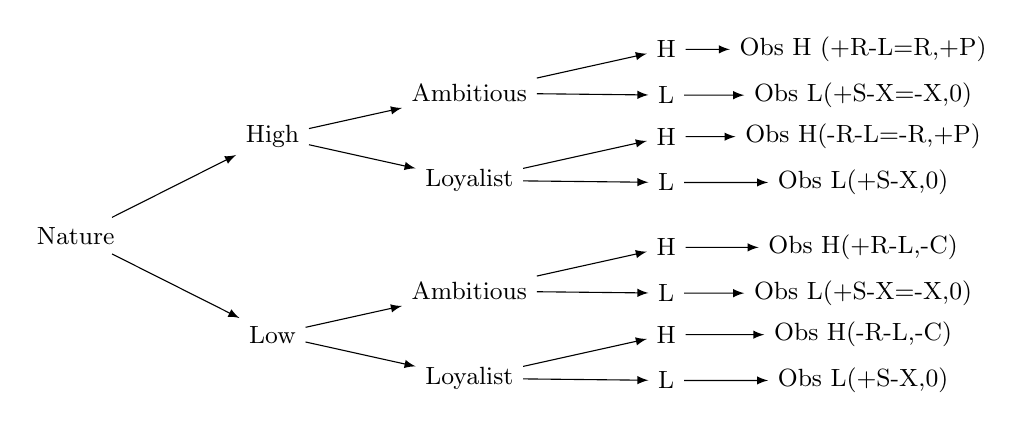
\begin{tikzpicture}[
      grow=right,
      level distance=25mm,
      sibling distance=10mm,
      every node/.style={font=\small, align=center},
      edge from parent/.style={draw, -latex}
    ]
    
    % Root node
    \node {Nature}
      % High productivity branch
      child [yshift=5em] {node {High}
        child [yshift=3em] {node {Ambitious}
          child [yshift=3em] {node {H}
            child {node {Obs H (+R-L=R,+P)}}
          }
          child [yshift=-1.5em] {node {L}
            child {node {Obs L(+S-X=-X,0)}}
          }
        }
        child [yshift=-3em] {node {Loyalist}
          child [yshift=3em] {node {H}
            child {node {Obs H(-R-L=-R,+P)}}
          }
          child [yshift=-1.5em] {node {L}
            child {node {Obs L(+S-X,0)}}
          }
        }
      }
      % Low productivity branch
      child [yshift=-5em] {node {Low}
        child [yshift=3em] {node {Ambitious}
          child [yshift=3em] {node {H}
            child {node {Obs H(+R-L,-C)}}
          }
          child [yshift=-1.5em] {node {L}
            child {node {Obs L(+S-X=-X,0)}}
          }
        }
        child [yshift=-3em] {node {Loyalist}
          child [yshift=3em] {node {H}
            child {node {Obs H(-R-L,-C)}}
          }
          child [yshift=-1.5em] {node {L}
            child {node {Obs L(+S-X,0)}}
          }
        }
      };
    
    \end{tikzpicture}
    \end{center}
High: High productivity commune leader\\
Low: Low productivity commune leader\\   
Ambitious: Ambitious commune leader who value promotion \\
Loyalist: Loyalist commune leader who value local interest\\
H: High contribution signaling\\
L: Low contribution signaling\\
L in payoff: cost of high contribution, positive for low type and zero for high type?\\
R: reward for high contribution and the promotion: positive for ambitious and negative for loyalist\\
S: reward for low contribution and trust from the commune members: zero for ambitious and positive for loyalist\\
P: reward for superior to make correct promotion\\
C: cost of promoting low type commune leader\\
X: placeholder for punishment for low contribution\\
\section{Model Households (Superstars)?}
We model highly visible but powerless households whose high effort levels influence others through social norms and imitation, rather than through redistribution authority. This extension is implemented using a scale-free network with behavioral spillovers from the central node.

\section{Conclusion}
Summary of insights from each model extension. Discussion of historical plausibility, policy relevance, and potential directions for further research.

\bibliographystyle{plainnat} % or abbrvnat, or plain
\bibliography{ref}  
\end{document}
